\documentclass[twocolumn]{article}
\usepackage{graphicx}
\usepackage{amsmath}
\usepackage{lipsum}
\usepackage{booktabs}
\usepackage{caption}
\captionsetup[table]{font=small, labelformat=empty}

\title{Vinum Analytica: Wine Review Insight}
\author{Paolo Palumbo}
\date{}

\begin{document}

\maketitle

\begin{abstract}
    This paper presents a data mining project that analyzes the language used in wine reviews written by sommeliers. We compare the performance of three different models: Decision Tree, Random Forest, and Neural Network. The analysis includes a detailed examination of preprocessing techniques, class contamination removal, and feature vectorization using TF-IDF. We assess the models based on their accuracy and present the results through various evaluations.
\end{abstract}

\section{Introduction}
The growing availability of online wine reviews provides a valuable resource for understanding consumer preferences and trends. This study aims to analyze the language used in these reviews to derive insights that can help in predicting wine ratings. We employ three machine learning models—Decision Tree, Random Forest, and Neural Network—to classify and predict wine ratings based on text features extracted from reviews.

\section{Preprocessing}
Data preprocessing is a critical step in any machine learning pipeline. In this project, we applied several preprocessing techniques to prepare the text data for modeling:

\begin{itemize}
    \item \textbf{Text Normalization:} All text was converted to lowercase to ensure uniformity.
    \item \textbf{Tokenization:} Text was split into individual words or tokens.
    \item \textbf{Stop Words Removal:} Common words that do not contribute to the semantic meaning were removed.
    \item \textbf{Stemming/Lemmatization:} Words were reduced to their base or root form.
\end{itemize}

\section{Feature Vectorization}
To transform the text data into a numerical format suitable for machine learning, we used the TF-IDF (Term Frequency-Inverse Document Frequency) method. This approach captures the importance of words in the context of the entire dataset and helps in feature extraction.

\section{Modeling and Hyperparameter Tuning}
We divided the dataset into training and test sets. The training set underwent oversampling using SMOTE to address class imbalance, with a limit of 200,000 records. We conducted a hyperparameter search using 6-fold cross-validation for each model to determine the best parameters based on accuracy.

\subsection{Decision Tree}
\begin{table}[h!]
    \centering
    \begin{tabular}{@{}cccc@{}}
        \toprule
        \textbf{Index} & \textbf{Criterion} & \textbf{Min Impurity Decrease} & \textbf{Max Depth} \\ \midrule
        0 & log\_loss & 0.0 & 1000 \\
        1 & entropy & 1e-12 & 1000 \\
        2 & gini & 0.0001 & 1000 \\
        3 & entropy & 0.0001 & None \\
        4 & entropy & 1e-12 & None \\
        5 & log\_loss & 0.0001 & None \\
        6 & gini & 1e-08 & 1000 \\
        7 & entropy & 1e-08 & 1000 \\ \bottomrule
    \end{tabular}
    \caption{Hyperparameters for Decision Tree}
\end{table}

\subsection{Random Forest}
\begin{table}[h!]
    \centering
    \begin{tabular}{@{}cccc@{}}
        \toprule
        \textbf{Index} & \textbf{n\_estimators} & \textbf{criterion} & \textbf{max\_depth} \\ \midrule
        0 & 150 & log\_loss & None \\
        1 & 50 & gini & None \\
        2 & 50 & gini & 1000 \\
        3 & 100 & entropy & None \\
        4 & 50 & entropy & None \\
        5 & 100 & gini & 1000 \\
        6 & 50 & log\_loss & None \\
        7 & 100 & gini & None \\ \bottomrule
    \end{tabular}
    \caption{Hyperparameters for Random Forest}
\end{table}

\subsection{Neural Network}
\begin{table}[h!]
    \centering
    \begin{tabular}{@{}cccc@{}}
        \toprule
        \textbf{Index} & \textbf{Hidden Size} & \textbf{Epochs} & \textbf{Learning Rate} \\ \midrule
        0 & 64 & 10 & 0.005 \\
        1 & 64 & 5 & 0.001 \\
        2 & 64 & 15 & 0.005 \\
        3 & 16 & 5 & 0.01 \\
        4 & 16 & 5 & 0.005 \\
        5 & 64 & 5 & 0.005 \\
        6 & 16 & 15 & 0.01 \\
        7 & 64 & 10 & 0.01 \\ \bottomrule
    \end{tabular}
    \caption{Hyperparameters for Neural Network}
\end{table}

\section{Results}
We evaluated the performance of the models using accuracy as the primary metric. The results for each model are presented through violin plots, which illustrate the distribution of accuracy scores across different hyperparameters.

\begin{figure}[h!]
    \centering
    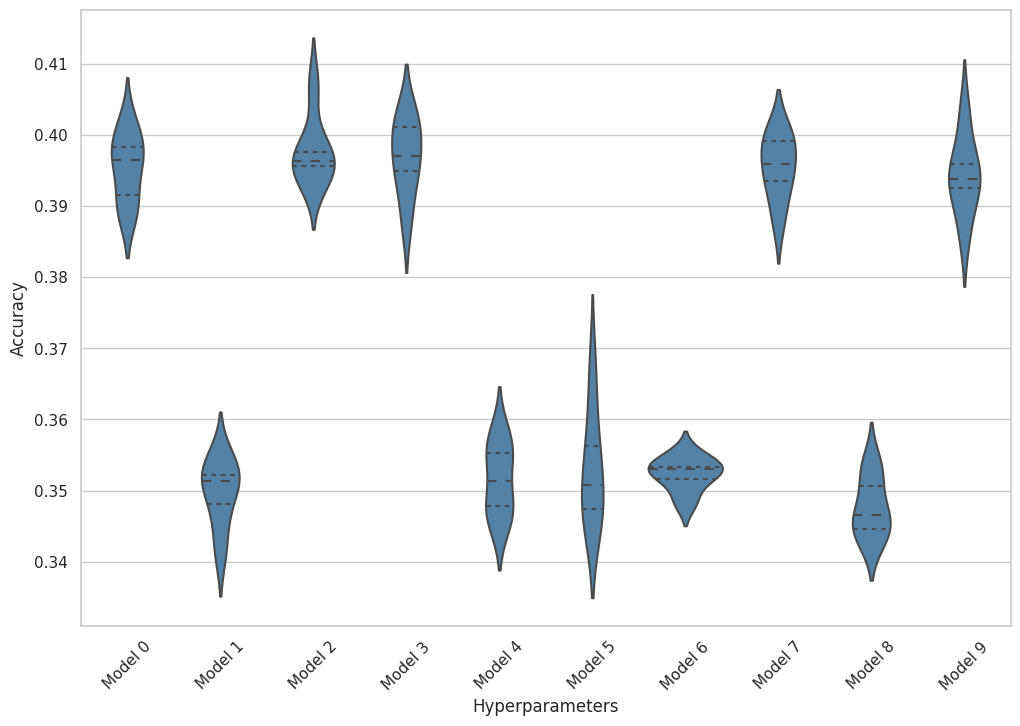
\includegraphics[width=\columnwidth]{images/violin_plot_decision_tree.png}
    \caption{Violin Plot for Decision Tree}
    \label{fig:decision_tree_violin}
\end{figure}

\begin{figure}[h!]
    \centering
    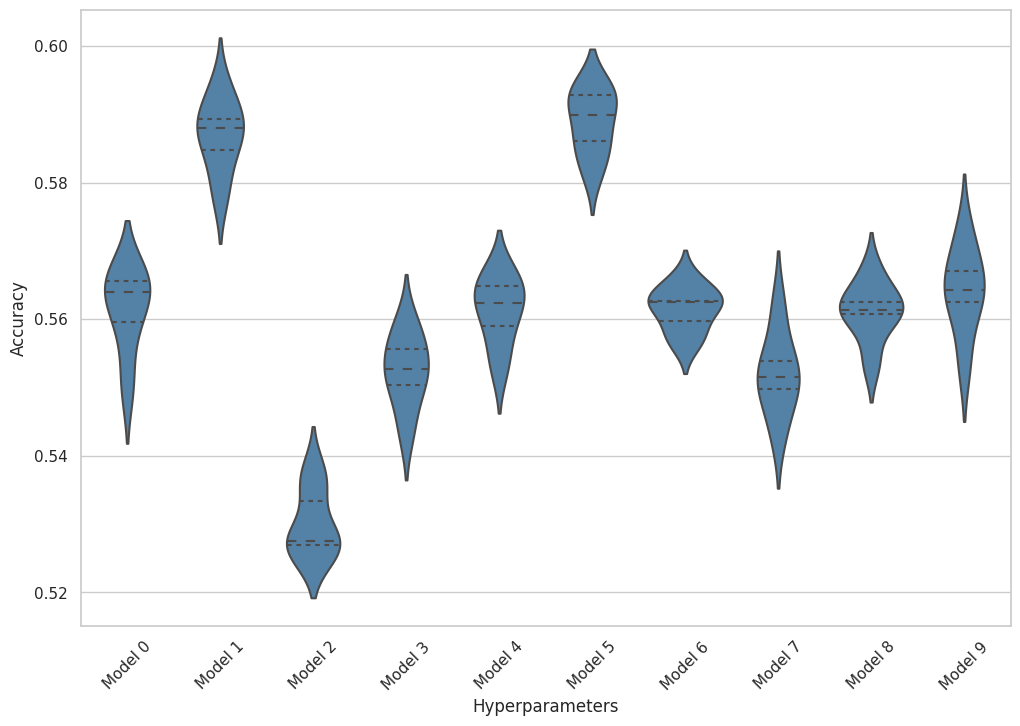
\includegraphics[width=\columnwidth]{images/violin_plot_random_forest.png}
    \caption{Violin Plot for Random Forest}
    \label{fig:random_forest_violin}
\end{figure}

\begin{figure}[h!]
    \centering
    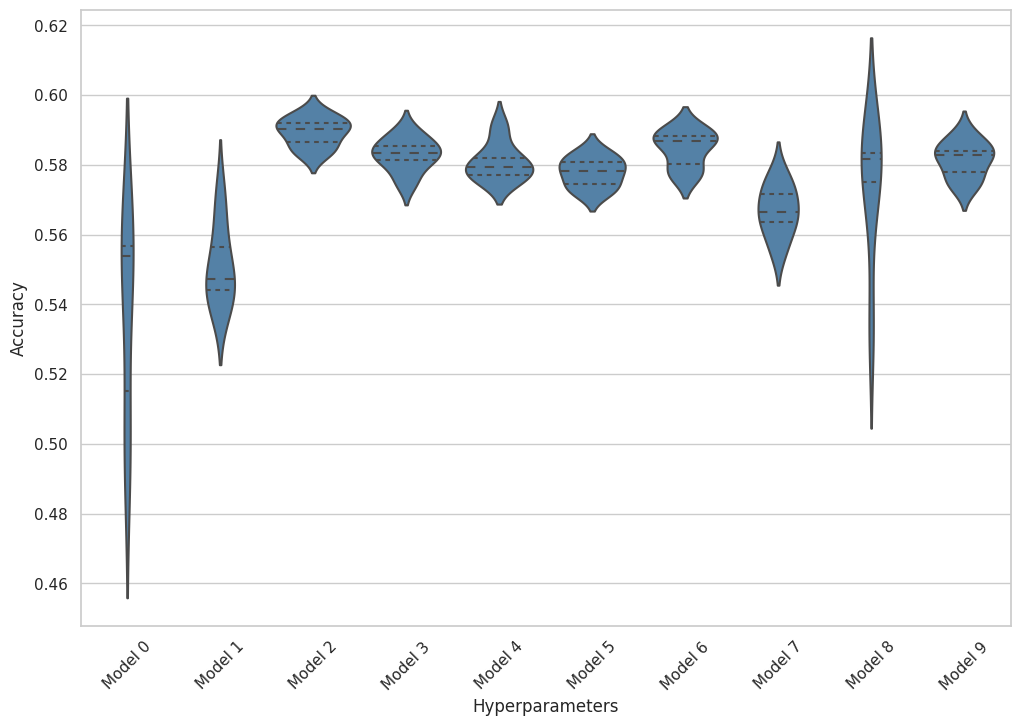
\includegraphics[width=\columnwidth]{images/violin_plot_neural_network.png}
    \caption{Violin Plot for Neural Network}
    \label{fig:neural_network_violin}
\end{figure}

\section{Discussion}
The analysis reveals the comparative performance of the Decision Tree, Random Forest, and Neural Network models in predicting wine ratings based on text reviews. The violin plots provide insights into the stability and variability of each model's accuracy across different hyperparameter settings. The Random Forest model generally showed the highest accuracy, followed by the Neural Network and Decision Tree models.

\section{Conclusion}
In this study, we have successfully compared three machine learning models for predicting wine ratings using text data. The Random Forest model demonstrated superior performance, while the Neural Network and Decision Tree models offered valuable insights as well. Future work could explore additional models and advanced preprocessing techniques to further improve prediction accuracy.

\end{document}
